% Options for packages loaded elsewhere
\PassOptionsToPackage{unicode}{hyperref}
\PassOptionsToPackage{hyphens}{url}
%
\documentclass[
]{article}
\usepackage{amsmath,amssymb}
\usepackage{iftex}
\ifPDFTeX
  \usepackage[T1]{fontenc}
  \usepackage[utf8]{inputenc}
  \usepackage{textcomp} % provide euro and other symbols
\else % if luatex or xetex
  \usepackage{unicode-math} % this also loads fontspec
  \defaultfontfeatures{Scale=MatchLowercase}
  \defaultfontfeatures[\rmfamily]{Ligatures=TeX,Scale=1}
\fi
\usepackage{lmodern}
\ifPDFTeX\else
  % xetex/luatex font selection
\fi
% Use upquote if available, for straight quotes in verbatim environments
\IfFileExists{upquote.sty}{\usepackage{upquote}}{}
\IfFileExists{microtype.sty}{% use microtype if available
  \usepackage[]{microtype}
  \UseMicrotypeSet[protrusion]{basicmath} % disable protrusion for tt fonts
}{}
\makeatletter
\@ifundefined{KOMAClassName}{% if non-KOMA class
  \IfFileExists{parskip.sty}{%
    \usepackage{parskip}
  }{% else
    \setlength{\parindent}{0pt}
    \setlength{\parskip}{6pt plus 2pt minus 1pt}}
}{% if KOMA class
  \KOMAoptions{parskip=half}}
\makeatother
\usepackage{xcolor}
\usepackage[margin=1in]{geometry}
\usepackage{color}
\usepackage{fancyvrb}
\newcommand{\VerbBar}{|}
\newcommand{\VERB}{\Verb[commandchars=\\\{\}]}
\DefineVerbatimEnvironment{Highlighting}{Verbatim}{commandchars=\\\{\}}
% Add ',fontsize=\small' for more characters per line
\usepackage{framed}
\definecolor{shadecolor}{RGB}{248,248,248}
\newenvironment{Shaded}{\begin{snugshade}}{\end{snugshade}}
\newcommand{\AlertTok}[1]{\textcolor[rgb]{0.94,0.16,0.16}{#1}}
\newcommand{\AnnotationTok}[1]{\textcolor[rgb]{0.56,0.35,0.01}{\textbf{\textit{#1}}}}
\newcommand{\AttributeTok}[1]{\textcolor[rgb]{0.13,0.29,0.53}{#1}}
\newcommand{\BaseNTok}[1]{\textcolor[rgb]{0.00,0.00,0.81}{#1}}
\newcommand{\BuiltInTok}[1]{#1}
\newcommand{\CharTok}[1]{\textcolor[rgb]{0.31,0.60,0.02}{#1}}
\newcommand{\CommentTok}[1]{\textcolor[rgb]{0.56,0.35,0.01}{\textit{#1}}}
\newcommand{\CommentVarTok}[1]{\textcolor[rgb]{0.56,0.35,0.01}{\textbf{\textit{#1}}}}
\newcommand{\ConstantTok}[1]{\textcolor[rgb]{0.56,0.35,0.01}{#1}}
\newcommand{\ControlFlowTok}[1]{\textcolor[rgb]{0.13,0.29,0.53}{\textbf{#1}}}
\newcommand{\DataTypeTok}[1]{\textcolor[rgb]{0.13,0.29,0.53}{#1}}
\newcommand{\DecValTok}[1]{\textcolor[rgb]{0.00,0.00,0.81}{#1}}
\newcommand{\DocumentationTok}[1]{\textcolor[rgb]{0.56,0.35,0.01}{\textbf{\textit{#1}}}}
\newcommand{\ErrorTok}[1]{\textcolor[rgb]{0.64,0.00,0.00}{\textbf{#1}}}
\newcommand{\ExtensionTok}[1]{#1}
\newcommand{\FloatTok}[1]{\textcolor[rgb]{0.00,0.00,0.81}{#1}}
\newcommand{\FunctionTok}[1]{\textcolor[rgb]{0.13,0.29,0.53}{\textbf{#1}}}
\newcommand{\ImportTok}[1]{#1}
\newcommand{\InformationTok}[1]{\textcolor[rgb]{0.56,0.35,0.01}{\textbf{\textit{#1}}}}
\newcommand{\KeywordTok}[1]{\textcolor[rgb]{0.13,0.29,0.53}{\textbf{#1}}}
\newcommand{\NormalTok}[1]{#1}
\newcommand{\OperatorTok}[1]{\textcolor[rgb]{0.81,0.36,0.00}{\textbf{#1}}}
\newcommand{\OtherTok}[1]{\textcolor[rgb]{0.56,0.35,0.01}{#1}}
\newcommand{\PreprocessorTok}[1]{\textcolor[rgb]{0.56,0.35,0.01}{\textit{#1}}}
\newcommand{\RegionMarkerTok}[1]{#1}
\newcommand{\SpecialCharTok}[1]{\textcolor[rgb]{0.81,0.36,0.00}{\textbf{#1}}}
\newcommand{\SpecialStringTok}[1]{\textcolor[rgb]{0.31,0.60,0.02}{#1}}
\newcommand{\StringTok}[1]{\textcolor[rgb]{0.31,0.60,0.02}{#1}}
\newcommand{\VariableTok}[1]{\textcolor[rgb]{0.00,0.00,0.00}{#1}}
\newcommand{\VerbatimStringTok}[1]{\textcolor[rgb]{0.31,0.60,0.02}{#1}}
\newcommand{\WarningTok}[1]{\textcolor[rgb]{0.56,0.35,0.01}{\textbf{\textit{#1}}}}
\usepackage{graphicx}
\makeatletter
\def\maxwidth{\ifdim\Gin@nat@width>\linewidth\linewidth\else\Gin@nat@width\fi}
\def\maxheight{\ifdim\Gin@nat@height>\textheight\textheight\else\Gin@nat@height\fi}
\makeatother
% Scale images if necessary, so that they will not overflow the page
% margins by default, and it is still possible to overwrite the defaults
% using explicit options in \includegraphics[width, height, ...]{}
\setkeys{Gin}{width=\maxwidth,height=\maxheight,keepaspectratio}
% Set default figure placement to htbp
\makeatletter
\def\fps@figure{htbp}
\makeatother
\setlength{\emergencystretch}{3em} % prevent overfull lines
\providecommand{\tightlist}{%
  \setlength{\itemsep}{0pt}\setlength{\parskip}{0pt}}
\setcounter{secnumdepth}{-\maxdimen} % remove section numbering
\ifLuaTeX
  \usepackage{selnolig}  % disable illegal ligatures
\fi
\IfFileExists{bookmark.sty}{\usepackage{bookmark}}{\usepackage{hyperref}}
\IfFileExists{xurl.sty}{\usepackage{xurl}}{} % add URL line breaks if available
\urlstyle{same}
\hypersetup{
  pdftitle={Introduction to Decision Trees in R},
  pdfauthor={Petros Pechlivanoglou},
  hidelinks,
  pdfcreator={LaTeX via pandoc}}

\title{Introduction to Decision Trees in R}
\usepackage{etoolbox}
\makeatletter
\providecommand{\subtitle}[1]{% add subtitle to \maketitle
  \apptocmd{\@title}{\par {\large #1 \par}}{}{}
}
\makeatother
\subtitle{3 vessel coronary artery disease (CAD) example}
\author{Petros Pechlivanoglou}
\date{Wednesday, September 13, 2023}

\begin{document}
\maketitle

\hypertarget{r-software}{%
\section{R software}\label{r-software}}

The R Project for Statistical Computing:
\url{https://www.r-project.org/}

\hypertarget{installing-r}{%
\section{Installing R}\label{installing-r}}

\emph{Install R}

Download R version 4.3.1 from
\url{https://cran.r-project.org/bin/windows/base/old/4.3.1/}

Download the file \texttt{R-4.3.1-win.exe} and follow the installation
procedure.

\emph{Install RStudio}

Download and install the free version of RStudio Desktop from:
\url{https://posit.co/download/rstudio-desktop/\#download}

\newpage

\hypertarget{building-a-tree}{%
\section{Building a Tree}\label{building-a-tree}}

This R Markdown document provides a foundation for constructing a
decision tree model for CAD:

Scenario - 70 yr old man with 3 vessel coronary artery disease (CAD).

\begin{Shaded}
\begin{Highlighting}[]
\FunctionTok{setwd}\NormalTok{(}\StringTok{"C:/Users/ppechlivanoglou/Documents/GitHub/Course{-}Modularization/static/Course\_Modularization/IHPME"}\NormalTok{)}
\NormalTok{knitr}\SpecialCharTok{::}\FunctionTok{include\_graphics}\NormalTok{(}\StringTok{"tree.png"}\NormalTok{)}
\end{Highlighting}
\end{Shaded}

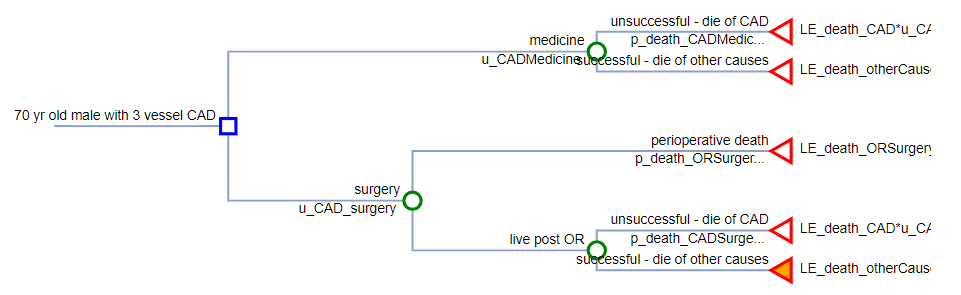
\includegraphics[width=13.35in]{tree} The two strategies being compared
are:

\begin{enumerate}
\def\labelenumi{\arabic{enumi}.}
\tightlist
\item
  Medical therapy
\item
  Surgery
\end{enumerate}

\begin{Shaded}
\begin{Highlighting}[]
\CommentTok{\# Unsuccessful medicine, die from CAD (probability) = 0.3}
\CommentTok{\# Life expectancy after unsuccessful medicine on CAD (life years) = 5}
\CommentTok{\# Life expectancy after successful medicine on CAD (life years) = 10}
\NormalTok{Medicine }\OtherTok{\textless{}{-}} \FloatTok{0.3} \SpecialCharTok{*} \DecValTok{5} \SpecialCharTok{+}\NormalTok{ (}\DecValTok{1} \SpecialCharTok{{-}} \FloatTok{0.3}\NormalTok{) }\SpecialCharTok{*} \DecValTok{10}
\NormalTok{Medicine}
\end{Highlighting}
\end{Shaded}

\begin{verbatim}
## [1] 8.5
\end{verbatim}

\begin{Shaded}
\begin{Highlighting}[]
\CommentTok{\# Perioperative death (probability) = 0.05}
\CommentTok{\# Life expectancy after perioperative death (life years) = 0}
\CommentTok{\# Unsuccessful surgery, die from CAD (probability) = 0.2}
\CommentTok{\# Life expectancy after unsuccessful surgery on CAD (life years) = 5}
\CommentTok{\# Life expectancy after successful surgery on CAD (life years) = 10}
\NormalTok{Surgery  }\OtherTok{\textless{}{-}} \FloatTok{0.05} \SpecialCharTok{*} \DecValTok{0} \SpecialCharTok{+}\NormalTok{ (}\DecValTok{1} \SpecialCharTok{{-}} \FloatTok{0.05}\NormalTok{) }\SpecialCharTok{*}\NormalTok{ (}\FloatTok{0.2} \SpecialCharTok{*} \DecValTok{5} \SpecialCharTok{+}\NormalTok{ (}\DecValTok{1} \SpecialCharTok{{-}} \FloatTok{0.2}\NormalTok{) }\SpecialCharTok{*} \DecValTok{10}\NormalTok{)}
\NormalTok{Surgery}
\end{Highlighting}
\end{Shaded}

\begin{verbatim}
## [1] 8.55
\end{verbatim}

This is an example of a tree built using NUMERIC values for
probabilities and ``payoffs''. The tree can be directly calculated to
yield an expected value - surgery is slightly preferred with an expected
value of 8.55 life years, compared with 8.50 life years for medicine.

Limited options, though, for sensitivity analysis.

\hypertarget{building-a-tree-with-variables}{%
\section{Building a Tree with
Variables}\label{building-a-tree-with-variables}}

Much greater flexibility is possible if numeric quantities in the tree
are defined as variables or expressions.

Variables can be globally defined and live in the Global Environment in
R and applied to the whole tree.

Steps for using variables:

\begin{enumerate}
\def\labelenumi{\arabic{enumi}.}
\tightlist
\item
  Declare name --- Based on its intended function in your model, decide
  on a clear name for the variable.
\item
  Use --- Anywhere the corresponding value is used in the tree (e.g.,
  payoffs or probabilities).
\end{enumerate}

Simplest way to create a variable is to type it in a R chunk like below:

\begin{Shaded}
\begin{Highlighting}[]
\CommentTok{\# Life expectancy (life years)}
\NormalTok{LE\_death\_CAD         }\OtherTok{\textless{}{-}} \DecValTok{5}    \CommentTok{\# Life expectancy after unsuccessful surgery on CAD}
\NormalTok{LE\_death\_ORSurgery   }\OtherTok{\textless{}{-}} \DecValTok{0}    \CommentTok{\# Life expectancy after perioperative death }
\NormalTok{LE\_death\_otherCauses }\OtherTok{\textless{}{-}} \DecValTok{10}   \CommentTok{\# Life expectancy after successful surgery on CAD }

\CommentTok{\# Probabilities}
\NormalTok{p\_death\_CADMedicine  }\OtherTok{\textless{}{-}} \FloatTok{0.3}  \CommentTok{\# Probability of death from CAD due to unsuccessful medicine}
\NormalTok{p\_death\_CADSurgery   }\OtherTok{\textless{}{-}} \FloatTok{0.2}  \CommentTok{\# Probability of death from CAD due to unsuccessful surgery}
\NormalTok{p\_death\_ORSurgery    }\OtherTok{\textless{}{-}} \FloatTok{0.05} \CommentTok{\# Probability of perioperative death}

\CommentTok{\# Utility (of CAD)}
\NormalTok{u\_CADMedicine        }\OtherTok{\textless{}{-}} \FloatTok{0.5}  \CommentTok{\# Utility after CAD under Medicine}
\NormalTok{u\_CADSurgery         }\OtherTok{\textless{}{-}} \FloatTok{0.8}  \CommentTok{\# Utility after CAD under Surgery}
\end{Highlighting}
\end{Shaded}

Our previous tree, now with variables:

\begin{Shaded}
\begin{Highlighting}[]
\NormalTok{Medicine }\OtherTok{\textless{}{-}}\NormalTok{     p\_death\_CADMedicine  }\SpecialCharTok{*}\NormalTok{ LE\_death\_CAD }\SpecialCharTok{+} 
\NormalTok{           (}\DecValTok{1} \SpecialCharTok{{-}}\NormalTok{ p\_death\_CADMedicine) }\SpecialCharTok{*}\NormalTok{ LE\_death\_otherCauses}
\NormalTok{Medicine}
\end{Highlighting}
\end{Shaded}

\begin{verbatim}
## [1] 8.5
\end{verbatim}

\begin{Shaded}
\begin{Highlighting}[]
\NormalTok{Surgery  }\OtherTok{\textless{}{-}}\NormalTok{     p\_death\_ORSurgery }\SpecialCharTok{*}\NormalTok{ LE\_death\_ORSurgery }\SpecialCharTok{+} 
\NormalTok{           (}\DecValTok{1} \SpecialCharTok{{-}}\NormalTok{ p\_death\_ORSurgery) }\SpecialCharTok{*}\NormalTok{ (      p\_death\_CADSurgery  }\SpecialCharTok{*}\NormalTok{ LE\_death\_CAD }\SpecialCharTok{+} 
\NormalTok{                                       (}\DecValTok{1} \SpecialCharTok{{-}}\NormalTok{ p\_death\_CADSurgery) }\SpecialCharTok{*}\NormalTok{ LE\_death\_otherCauses}
\NormalTok{                                     )}
\NormalTok{Surgery}
\end{Highlighting}
\end{Shaded}

\begin{verbatim}
## [1] 8.55
\end{verbatim}

Now, among other things, sensitivity analysis is possible.

\begin{Shaded}
\begin{Highlighting}[]
\NormalTok{v\_p\_death\_ORSurgery }\OtherTok{\textless{}{-}} \FunctionTok{c}\NormalTok{(}\DecValTok{0}\NormalTok{, }\FloatTok{0.1}\NormalTok{, }\FloatTok{0.2}\NormalTok{, }\FloatTok{0.3}\NormalTok{, }\FloatTok{0.4}\NormalTok{, }\FloatTok{0.5}\NormalTok{, }\FloatTok{0.6}\NormalTok{, }\FloatTok{0.7}\NormalTok{, }\FloatTok{0.8}\NormalTok{, }\FloatTok{0.9}\NormalTok{, }\DecValTok{1}\NormalTok{)}
\CommentTok{\# v\_p\_death\_ORSurgery \textless{}{-} seq(0, 1, 0.1) \# simpler}
\NormalTok{Medicine\_sens }\OtherTok{\textless{}{-}}\NormalTok{     p\_death\_CADMedicine  }\SpecialCharTok{*}\NormalTok{ LE\_death\_CAD }\SpecialCharTok{+} 
\NormalTok{                (}\DecValTok{1} \SpecialCharTok{{-}}\NormalTok{ p\_death\_CADMedicine) }\SpecialCharTok{*}\NormalTok{ LE\_death\_otherCauses}

\NormalTok{Surgery\_sens  }\OtherTok{\textless{}{-}}\NormalTok{     v\_p\_death\_ORSurgery  }\SpecialCharTok{*}\NormalTok{ LE\_death\_ORSurgery }\SpecialCharTok{+} 
\NormalTok{                (}\DecValTok{1} \SpecialCharTok{{-}}\NormalTok{ v\_p\_death\_ORSurgery) }\SpecialCharTok{*}\NormalTok{ (      p\_death\_CADSurgery  }\SpecialCharTok{*}\NormalTok{ LE\_death\_CAD }\SpecialCharTok{+} 
\NormalTok{                                              (}\DecValTok{1} \SpecialCharTok{{-}}\NormalTok{ p\_death\_CADSurgery) }\SpecialCharTok{*}\NormalTok{ LE\_death\_otherCauses}
\NormalTok{                                            )}
\FunctionTok{plot}\NormalTok{(v\_p\_death\_ORSurgery, Surgery\_sens, }\AttributeTok{type=}\StringTok{"l"}\NormalTok{, }\AttributeTok{main=}\StringTok{"Sensitivity Analysis"}\NormalTok{, }
     \AttributeTok{xlab=}\StringTok{"probability of perioperative death"}\NormalTok{, }\AttributeTok{ylab=}\StringTok{"Expected value"}\NormalTok{, }\AttributeTok{col=}\StringTok{"red"}\NormalTok{)}
\FunctionTok{points}\NormalTok{(v\_p\_death\_ORSurgery, Surgery\_sens, }\AttributeTok{col=}\StringTok{"red"}\NormalTok{)}
\FunctionTok{lines}\NormalTok{(v\_p\_death\_ORSurgery, }\FunctionTok{rep}\NormalTok{(Medicine\_sens, }\DecValTok{11}\NormalTok{), }\AttributeTok{col=}\StringTok{"blue"}\NormalTok{)}
\FunctionTok{points}\NormalTok{(v\_p\_death\_ORSurgery, }\FunctionTok{rep}\NormalTok{(Medicine\_sens, }\DecValTok{11}\NormalTok{), }\AttributeTok{col=}\StringTok{"blue"}\NormalTok{)}
\FunctionTok{legend}\NormalTok{(}\StringTok{"right"}\NormalTok{, }\FunctionTok{c}\NormalTok{(}\StringTok{"Medicine"}\NormalTok{, }\StringTok{"Surgery"}\NormalTok{), }\AttributeTok{col=}\FunctionTok{c}\NormalTok{(}\StringTok{"blue"}\NormalTok{, }\StringTok{"red"}\NormalTok{), }\AttributeTok{lty=}\FunctionTok{c}\NormalTok{(}\DecValTok{1}\NormalTok{,}\DecValTok{1}\NormalTok{), }\AttributeTok{bty=}\StringTok{"n"}\NormalTok{)}
\end{Highlighting}
\end{Shaded}

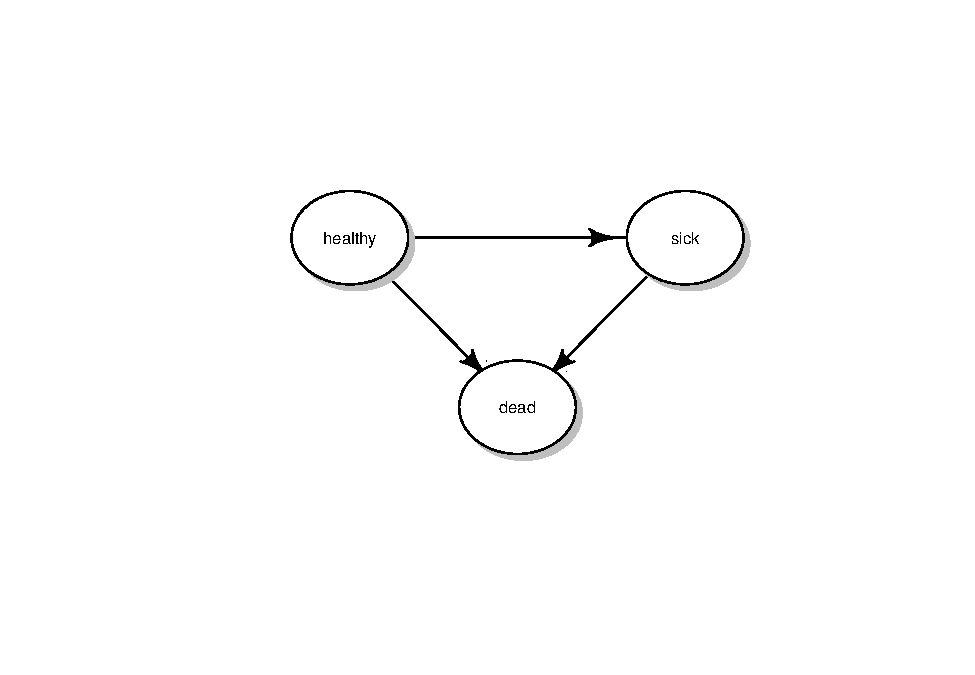
\includegraphics{decision_tree_class_new_files/figure-latex/unnamed-chunk-5-1.pdf}

\hypertarget{using-subtrees}{%
\section{Using Subtrees}\label{using-subtrees}}

In R you can create subtrees and assign them to functions with desired
names. For example, the subtree describing outcomes for those alive post
OR can be assigned into a function and we can call it
\texttt{Effectiveness\_Subtree}. The arguments of this function include
probability of death if treatment is unsuccessful, life expectancy if
treatment is unsuccessful and successful, and utility after CAD. We
assume utilities for those with successful treatment to have a utility
of 1.

\begin{Shaded}
\begin{Highlighting}[]
\CommentTok{\# p\_death\_Tx: probability of death after unsuccessful treatment}
\CommentTok{\# LE\_death\_Tx: life expectancy after unsuccessful treatment}
\CommentTok{\# LE\_death\_noTx: life expectancy after successful treatment}
\CommentTok{\# u\_CAD: utility after CAD}
\NormalTok{Effectiveness\_Subtree }\OtherTok{\textless{}{-}} \ControlFlowTok{function}\NormalTok{(p\_death\_Tx, LE\_death\_Tx, LE\_death\_noTx, u\_CAD) \{}
  
\NormalTok{                                      p\_death\_Tx  }\SpecialCharTok{*}\NormalTok{ LE\_death\_Tx   }\SpecialCharTok{*}\NormalTok{ u\_CAD }\SpecialCharTok{+} 
\NormalTok{                                 (}\DecValTok{1} \SpecialCharTok{{-}}\NormalTok{ p\_death\_Tx) }\SpecialCharTok{*}\NormalTok{ LE\_death\_noTx }\SpecialCharTok{*} \DecValTok{1}
\NormalTok{\}}
\end{Highlighting}
\end{Shaded}

To use this subtree function, you just need to pass values to the
arguments. Below we calculate QALY outcomes for both medicine and
surgery while using subtree \texttt{Effectiveness\_Subtree} for both
strategies.

\begin{Shaded}
\begin{Highlighting}[]
\NormalTok{Medicine }\OtherTok{\textless{}{-}} \FunctionTok{Effectiveness\_Subtree}\NormalTok{(}\AttributeTok{p\_death\_Tx    =}\NormalTok{ p\_death\_CADMedicine, }
                                  \AttributeTok{LE\_death\_Tx   =}\NormalTok{ LE\_death\_CAD, }
                                  \AttributeTok{LE\_death\_noTx =}\NormalTok{ LE\_death\_otherCauses, }
                                  \AttributeTok{u\_CAD         =}\NormalTok{ u\_CADMedicine)}
\NormalTok{Medicine}
\end{Highlighting}
\end{Shaded}

\begin{verbatim}
## [1] 7.75
\end{verbatim}

\begin{Shaded}
\begin{Highlighting}[]
\NormalTok{Surgery  }\OtherTok{\textless{}{-}}\NormalTok{      p\_death\_ORSurgery  }\SpecialCharTok{*}\NormalTok{ LE\_death\_ORSurgery }\SpecialCharTok{+}  
\NormalTok{            (}\DecValTok{1} \SpecialCharTok{{-}}\NormalTok{ p\_death\_ORSurgery) }\SpecialCharTok{*} \FunctionTok{Effectiveness\_Subtree}\NormalTok{(}\AttributeTok{p\_death\_Tx    =}\NormalTok{ p\_death\_CADSurgery, }
                                                            \AttributeTok{LE\_death\_Tx   =}\NormalTok{ LE\_death\_CAD, }
                                                            \AttributeTok{LE\_death\_noTx =}\NormalTok{ LE\_death\_otherCauses, }
                                                            \AttributeTok{u\_CAD         =}\NormalTok{ u\_CADSurgery)}
\NormalTok{Surgery}
\end{Highlighting}
\end{Shaded}

\begin{verbatim}
## [1] 8.36
\end{verbatim}

\end{document}
